The unit card shows the current capabilities of a trooper and tracks damage.
A unit card can be formatted in any way so long as it contains all the essential information.
Below is a sample unit card for a basic infantry trooper.

\begin{figure}[H]
  \centering
  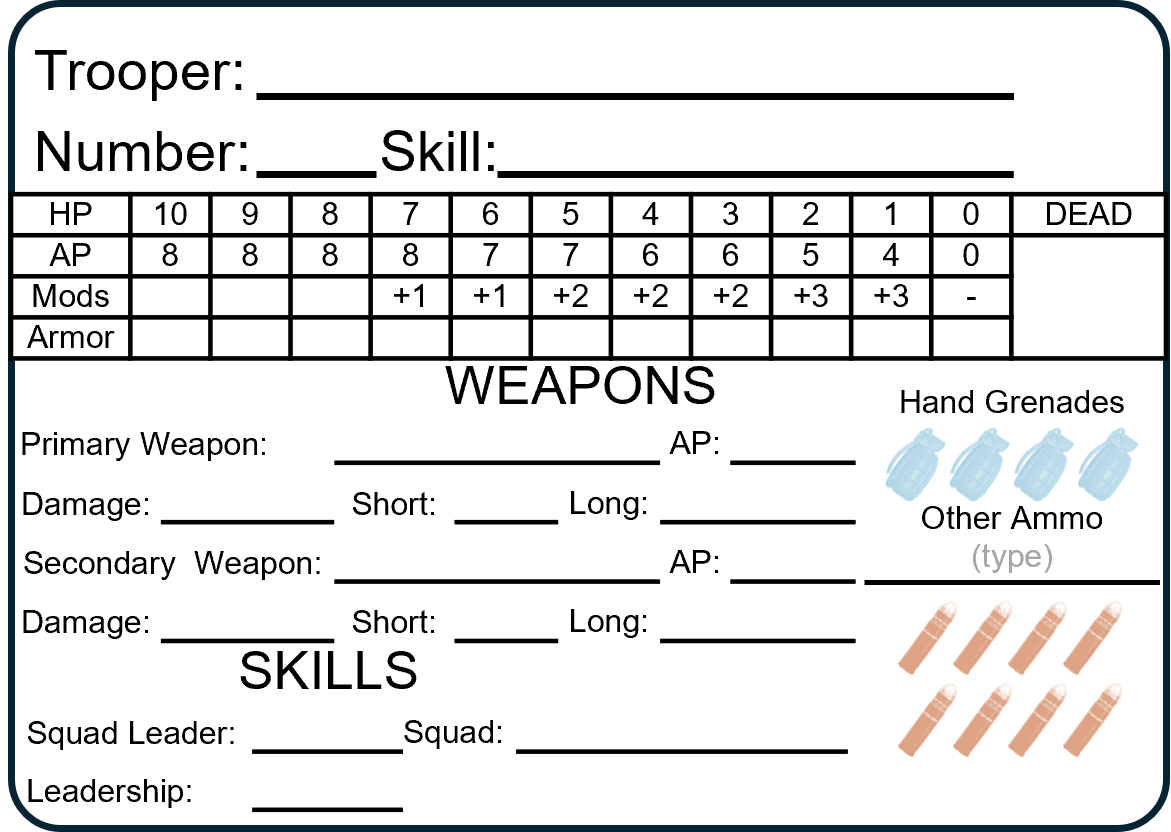
\includegraphics[alt='Sample Regular Trooper', width=5.63in, height=4in]{img/RegularTrooper.png}
  \caption*{Basic Regular Trooper Unit Card}
\end{figure}

Basic information about the trooper, such as their name, rank, squad position number, and skill level are tracked at the top of the unit card.

Damage to the trooper is tracked in the HP section.
HP cells are labeled by their HP value, from highest to lowest, 10 to 1, from left to right.
HP cells are fully crossed out when the trooper takes lethal damage (X) and partially crossed out when the trooper takes bludgeoning damage (\textbackslash).
The current HP of the trooper is given by the first cell to the right of the lowest fully crossed out HP cell.
For example, if the trooper has HP 9, 7, and 6 fully crossed out and HP 5 partially crossed out, then their current HP is 5.

Total action points (AP) for the trooper are given in the AP section.
Use the value in the column corresponding to the trooper's current HP.
For example, if the trooper has 5 HP, then they have 7 AP.

Similarly, the modifier section tracks the current modifier for the trooper's target numbers based upon current HP.
For example, if the trooper has 5 HP, then add +2 to all target numbers.

If the trooper is wearing armor, mark the contiguous block of HP cells protected by the armor in the Armor section.
Armor must be destroyed before the corresponding HP cell is marked off.

The weapons and equipment section list the primary and secondary weapons the trooper is carrying, along with their damage values and range brackets.
Basic troopers also carry 4 hand grenades and may carry additional equipment.
Any rifle automatically comes with a bayonet equipped.

The leadership section lists the squad leader for the trooper and their leadership score.
This section contains the information required for morale checks.
